\chapter{Theoredical Background}\label{chap:theoredical_background}

\begin{toreview}

	\gls{ai} safety is a very broad term that is fuzzily defined, this section will explore the history of the field compartmentalize it into several digestible areas. This is a theoretical foundation that will tackle all the most common \gls{ai} safety terms and terminology that will be tackled across this work.

	% - Orthogonality Thesis
	% - Instrumental Convergence
	% - Inner and Outter aligment
	% - Maximizers and Satisfizers
	% - Reward Hacking
	% - Aligment Faking
	% - ELK (Eliciit Latent Knowledge)
	% - Explainability
	% Podes olhar para o algiment research center: https://www.alignment.org/blog/a-birds-eye-view-of-arcs-research/
	% Article: Artificial Intelligence: Approaches to Safety (REFERENCE WITH: \cite{DAlessandro2025})

	\section{The Evolution of AI Safety}

	The evolution of the field can be roughly divided into three distinct eras: A Speculative Era (Pre-2010), the move towards Engineering Solutions (2010 -- 2014), Mainstream Attention and Existential Risk (2014 -- Present). The timeline is illustrated in Figure \ref{fig:ai_safety_timeline}.

	% template from https://www.overleaf.com/latex/templates/timeline/fswhyzqjhhbc
\begin{figure}[htpb]
    \centering
    % This resizebox forces the timeline to fit exactly within the page margins.
    \resizebox{\textwidth}{!}{
    
    \begin{tikzpicture}[font=\small]
    
        % --- Styles ---
        \tikzset{
            era_box/.style={align=center, font=\footnotesize\bfseries},
            % Style for events above the axis
            event_top/.style={draw=#1, fill=#1!5, thick, rounded corners=3pt, align=center, text width=2.5cm, font=\scriptsize, inner sep=4pt, anchor=south},
            % Style for events below the axis
            event_bot/.style={draw=#1, fill=#1!5, thick, rounded corners=3pt, align=center, text width=2.5cm, font=\scriptsize, inner sep=4pt, anchor=north},
            % Arrow styles
            arrow_top/.style={-{Latex[length=1.5mm, width=1.5mm]}, thick, #1},
            arrow_bot/.style={-{Latex[length=1.5mm, width=1.5mm]}, thick, #1},
        }
    
        % --- Variables ---
        \def\h{1.4} % Height of the Era background boxes
    
        % --- Color Definitions (Blue + Yellow = Green) ---
        % Era 1: Blue
        \definecolor{Era1Fill}{RGB}{230, 242, 255} % Very pale blue
        \definecolor{Era1Line}{RGB}{0, 102, 204}   % Deep academic blue
        
        % Era 2: Yellow
        \definecolor{Era2Fill}{RGB}{255, 252, 230} % Very pale yellow
        \definecolor{Era2Line}{RGB}{184, 134, 11}  % Deep goldenrod/mustard (for readability)
        
        % Era 3: Green
        \definecolor{Era3Fill}{RGB}{235, 247, 235} % Very pale green
        \definecolor{Era3Line}{RGB}{34, 139, 34}   % Deep forest green
    
        % --- Era Background Rectangles ---
        \shade[top color=Era1Fill!60, bottom color=Era1Fill] (0,0) rectangle (4.8,\h);
        \shade[top color=Era2Fill!60, bottom color=Era2Fill] (4.8,0) rectangle (9.2,\h);
        \shade[top color=Era3Fill!60, bottom color=Era3Fill] (9.2,0) rectangle (15.2,\h);
    
        % --- Era Labels ---
        \node[era_box, text=Era1Line] at (2.4, \h/2) {Speculative Era};
        \node[era_box, text=Era2Line] at (7.0, \h/2) {Engineering\\Solutions};
        \node[era_box, text=Era3Line] at (12.2, \h/2) {Mainstream \&\\Existential Risk};
    
        % --- Main Axis Line ---
        \draw[line width=1.5pt, draw=black!80] (0,0) -- (0.8,0);
        \draw[->, >=Latex, line width=1.5pt, draw=black!80] (1.2,0) -- (15.5,0) node[right, font=\footnotesize\bfseries] {};
    
        % --- Axis Break Symbol (To skip from 1949 to 2000s) ---
        \draw[line width=1.2pt, draw=black!80] (0.9,-0.2) -- (1.1,0.2);
        \draw[line width=1.2pt, draw=black!80] (0.7,-0.2) -- (0.9,0.2);
    
        % ==========================================
        % EVENTS PLACEMENT
        % ==========================================
        
        % --- ERA 1: Pre-2010 (BLUE) ---
        
        % 1949 (Bottom)
        \def\x{0.3}
        \draw[draw=black!70, thick] (\x, 0) -- (\x, -0.1);
        \node[event_bot=Era1Line] (E1) at (\x, -0.5) {\textbf{1949}\\Wiener warns of machine defiance};
        \draw[arrow_bot=Era1Line] (E1.north) -- (\x, -0.1);
    
        % 2001 (Top)
        \def\x{2.2}
        \draw[draw=black!70, thick] (\x, \h) -- (\x, \h+0.1);
        \node[event_top=Era1Line] (E2) at (\x, \h+0.5) {\textbf{2001}\\Singularity Institute (MIRI) founded};
        \draw[arrow_top=Era1Line] (E2.south) -- (\x, \h+0.1);
    
        % 2008 (Bottom)
        \def\x{4.2}
        \draw[draw=black!70, thick] (\x, 0) -- (\x, -0.1);
        \node[event_bot=Era1Line] (E3) at (\x, -0.5) {\textbf{2008}\\Omohundro:\\\textit{Basic AI Drives}};
        \draw[arrow_bot=Era1Line] (E3.north) -- (\x, -0.1);
    
    
        % --- ERA 2: 2011 - 2016 (YELLOW/GOLD) ---
    
        % 2011 (Top)
        \def\x{5.5}
        \draw[draw=black!70, thick] (\x, \h) -- (\x, \h+0.1);
        \node[event_top=Era2Line] (E4) at (\x, \h+0.5) {\textbf{2011}\\Yampolskiy:\\AI Safety Engineering};
        \draw[arrow_top=Era2Line] (E4.south) -- (\x, \h+0.1);
    
        % 2014 (Bottom)
        \def\x{7.0}
        \draw[draw=black!70, thick] (\x, 0) -- (\x, -0.1);
        \node[event_bot=Era2Line] (E5) at (\x, -0.5) {\textbf{2014}\\Bostrom publishes\\\textit{Superintelligence}};
        \draw[arrow_bot=Era2Line] (E5.north) -- (\x, -0.1);
    
        % 2016 (Top)
        \def\x{8.5}
        \draw[draw=black!70, thick] (\x, \h) -- (\x, \h+0.1);
        \node[event_top=Era2Line] (E6) at (\x, \h+0.5) {\textbf{2016}\\\textit{Concrete Problems in AI Safety}};
        \draw[arrow_top=Era2Line] (E6.south) -- (\x, \h+0.1);
    
    
        % --- ERA 3: 2017 - 2025 (GREEN) ---
    
        % 2017 (Bottom)
        \def\x{10.0}
        \draw[draw=black!70, thick] (\x, 0) -- (\x, -0.1);
        \node[event_bot=Era3Line] (E7) at (\x, -0.5) {\textbf{2017}\\Asilomar Conf. on Beneficial AI};
        \draw[arrow_bot=Era3Line] (E7.north) -- (\x, -0.1);
    
        % 2021 (Top)
        \def\x{11.6}
        \draw[draw=black!70, thick] (\x, \h) -- (\x, \h+0.1);
        \node[event_top=Era3Line] (E8) at (\x, \h+0.5) {\textbf{2021}\\\textit{Unsolved Problems in ML Safety}};
        \draw[arrow_top=Era3Line] (E8.south) -- (\x, \h+0.1);
    
        % 2023 (Bottom)
        \def\x{13.2}
        \draw[draw=black!70, thick] (\x, 0) -- (\x, -0.1);
        \node[event_bot=Era3Line] (E9) at (\x, -0.5) {\textbf{2023}\\1st Global AI\\Safety Summit};
        \draw[arrow_bot=Era3Line] (E9.north) -- (\x, -0.1);
    
        % 2025 (Top)
        \def\x{14.8}
        \draw[draw=black!70, thick] (\x, \h) -- (\x, \h+0.1);
        \node[event_top=Era3Line] (E10) at (\x, \h+0.5) {\textbf{2025}\\First Intl. AI\\Safety Report};
        \draw[arrow_top=Era3Line] (E10.south) -- (\x, \h+0.1);
    
    \end{tikzpicture}
    
    } % End of resizebox
    \caption{Timeline of the evolution of the AI Safety field.}
    \label{fig:ai_safety_timeline}
\end{figure}

	\subsection{Speculative Era}

	Risks from \gls{ai} were discussed early on, with Norbert Wiener warning of machine defiance in 1949 \cite{wiener1950}. Before 2010, the field remained largely theoretical, focusing on philosophy and machine ethics \cite{whitby1988}. An early institutional milestone was the founding of the Singularity Institute for Artificial Intelligence (later renamed MIRI) in 2001 \cite{yudkowsky2001friendly}, one of the first organisations dedicated exclusively to researching safe and beneficial AI. A critical milestone was Steve Omohundro's 2008 paper on "Basic AI Drives" \cite{omohundro2008basic}. This established the theoretical roots of Instrumental Convergence (see Section \ref{sec:foundations}), arguing that optimizing agents naturally develop dangerous sub-goals, such as resource acquisition, regardless of their initial programming.

	\subsection{Move towards Engineering Solutions}

	A pivotal shift occurred in 2011 when Roman Yampolskiy introduced the term "AI safety engineering" \cite{yampolskiy2011, yampolskiy_controllability_2022}. The field transitioned from asking "What should an AI want?" to building provably safe, controllable systems using methodologies from cybersecurity and control theory \cite{control_theory_safety}. This engineering mindset was solidified by the 2016 publication of \textit{Concrete Problems in AI Safety} \cite{amodei2016concrete}, an influential agenda that formally outlined technical issues like reward hacking and safe exploration. DeepMind further formalized the field in 2018 by proposing a taxonomy of three technical safety pillars: Specification, Robustness, and Assurance. This became a canonical reference for safety engineering research \cite{ortega2018building}.

	\subsection{Mainstreaming and Existential Risk}

	Nick Bostrom's 2014 book \textit{Superintelligence} \cite{bostrom2014superintelligence} brought AI safety concerns, namely,  Existential Risk and the Control Problem, into mainstream discourse; prompting prominent tech figures like Elon Musk, Bill Gates, and Stephen Hawking to voice similar concerns. This drove significant funding into safety institutions. In 2015, the \gls{fli} awarded \$6.5 million in grants for beneficial \gls{ai} research. \end{toreview} The 2017 Asilomar Conference on Beneficial AI produced 23 governance principles signed by over 1,700 AI researchers, representing the field's first broad normative consensus \cite{futureoflife2017asilomar}. As deep learning accelerated, experts increasingly debated the probability of these civilizational threats \cite{field_why_2025}, and Hendrycks et al. updated the technical roadmap with \textit{Unsolved Problems in ML Safety} \cite{hendrycks2021unsolved}, identifying Robustness, Monitoring, Alignment, and Systemic Safety as open research directions. In March 2023, the \gls{fli} called for a six-month moratorium on training AI systems more powerful than GPT-4, gathering over 30,000 signatures and catalyzing global debate on AI risk \cite{futureoflife2023pause}. Recently, safety has reached global governance, with the first Global AI Safety Summit held at Bletchley Park in late 2023, a bilateral AI safety partnership formalized between the UK and the US in 2024 \cite{ukus2024mou}, and the 2025 International \gls{ai} Safety Report, which represents an effort from the UK government to review \gls{ai} risks \cite{AISafetyReport2025}.


\begin{reviewed}

\section{The Alignment Problem}\label{sec:alignment-problem}

	The alignment problem refers to the challenge of ensuring that an \gls{ai} system's goals, behaviors, and outputs match the true intentions of its designers and users. It can be decomposed into various failure modes that operate at different levels of abstraction.

	\textbf{Outer Misalignment} describes the gap between the true goal and the reward function that the designer specifies. Key phenomena here include Reward Hacking (also called Specification Gaming), where the agent finds a loophole to score high rewards without completing the intended task \cite{amodei2016concrete, skalse2022defining}, and its extreme form, Wireheading, where the agent directly manipulates its own reward signal \cite{everitt2021reward}. Underpinning both is Goodhart's Law \cite{manheim2019categorizing, langlois2024goodhart}: once a measure becomes a target, it ceases to be a good measure.

	\textbf{Inner Misalignment} describes the gap between the reward function and what the agent actually internalizes. Its root cause is Mesa-Optimization: when a trained model is itself a learning
	algorithm \cite{hubinger2019risks} (see Figure~\ref{fig:mesa-optimisation-chain}), it may develop an internal mesa-objective that diverges from the training objective. Goal Misgeneralisation is a downstream symptom, where the learned goal holds during training but breaks down under distributional shift.

	% ============================================================
%  Mesa-Optimisation Chain — Figure + Comparison Table
%  Insert after the Alignment Problem section (or wherever fits)
%  Requires: tikz (calc, arrows.meta, positioning, shapes.misc),
%            booktabs, threeparttable  [all loaded in preamble.sty]
% ============================================================

% ------------------------------------------------------------------
%  FIGURE: Mesa-Optimisation Chain
% ------------------------------------------------------------------
\begin{figure}[htbp]
\centering
\begin{tikzpicture}[
    >=Stealth,
    line width=0.8pt,
    font=\small,
    bigbox/.style={
        draw, rectangle,
        minimum width=3.2cm, minimum height=4.0cm,
        line width=1.0pt
    },
    objbox/.style={
        draw, rectangle,
        minimum width=2.5cm, minimum height=0.75cm,
        line width=0.8pt, align=center, font=\footnotesize
    },
    mainarrow/.style={->, line width=0.9pt},
    dasharrow/.style={ ->, dashed, line width=0.8pt},
]

% ----------------------------------------------------------------
%  A) HUMAN — circle labelled "Human" with tiny stick body below
% ----------------------------------------------------------------
\node[
    circle, draw, fill=white,
    minimum size=1.5cm, inner sep=2pt,
    align=center, font=\small\bfseries,
    line width=0.9pt
] (human) at (0, 2.6) {Human};

% Tiny stick body hanging below the circle
\coordinate (torsoTop) at (0, 1.82);
\coordinate (torsoBot) at (0, 1.30);
\draw[line width=0.55pt] (torsoTop) -- (torsoBot);
\draw[line width=0.55pt] (0, 1.65) -- (-0.25, 1.40);  % left arm
\draw[line width=0.55pt] (0, 1.65) -- ( 0.25, 1.40);  % right arm
\draw[line width=0.55pt] (torsoBot) -- (-0.20, 0.90);  % left leg
\draw[line width=0.55pt] (torsoBot) -- ( 0.20, 0.90);  % right leg

% ----------------------------------------------------------------
%  B) OBJECTIVE BADGE — circle to the RIGHT of Human
% ----------------------------------------------------------------
\node[
    circle, draw, fill=white,
    minimum size=1.3cm, inner sep=1pt,
    align=center, font=\footnotesize\bfseries,
    line width=0.8pt
] (humobj) at (2.0, 2.6) {Objective};

% Short connector line: human → objective badge
\draw[line width=0.5pt] (human.east) -- (humobj.west);

% ----------------------------------------------------------------
%  C) BASE OPTIMIZER BOX  (centered at x=5.4)
% ----------------------------------------------------------------
\node[bigbox] (baseopt) at (5.4, 2.10) {};
\node[above, font=\small\bfseries, anchor=south] at (baseopt.north)
    {Base Optimizer};

\node[objbox] (baseobj) at (5.4, 0.82)
    {(BASE) Objective};

% ----------------------------------------------------------------
%  D) MODEL (MESA-OPTIMIZER) BOX  (centered at x=10.0)
% ----------------------------------------------------------------
\node[bigbox] (model) at (10.0, 2.10) {};
\node[above, align=center, font=\small\bfseries, anchor=south] at (model.north)
    {Model\\[-3pt]\normalfont\scriptsize(Mesa-Optimizer)};

\node[objbox] (mesaobj) at (10.0, 0.82)
    {(mesa) Objective};

% ----------------------------------------------------------------
%  E) WORLD — circle with dashed equator and meridian
% ----------------------------------------------------------------
\node[
    circle, draw, fill=white,
    minimum size=1.8cm, inner sep=2pt,
    align=center, font=\small\bfseries,
    line width=0.9pt
] (world) at (13.8, 2.10) {World};

% Dashed equator
\draw[dashed, line width=0.55pt]
    (13.8, 2.10) ellipse (0.90cm and 0.25cm);
% Dashed meridian
\draw[dashed, line width=0.55pt]
    (13.8, 2.10) ellipse (0.25cm and 0.90cm);

% ----------------------------------------------------------------
%  F) ARROWS
% ----------------------------------------------------------------

% 1. Outer Alignment — dashed: Objective badge → BASE Objective box
\draw[dasharrow]
    (humobj.south)
    to[out=-80, in=175]
    node[
        pos=0.48,
        below, sloped,
        font=\scriptsize
    ] {Outer Alignment}
    (baseobj.west);

% 2. Optimizes — top-level: Base Optimizer → Model
\draw[mainarrow]
    ([yshift=0.55cm] baseopt.east)
    --
    node[above, font=\scriptsize] {Optimizes}
    ([yshift=0.55cm] model.west);

% 3. Inner Alignment — lower-level: BASE Obj → mesa Obj
\draw[mainarrow]
    (baseobj.east)
    --
    node[above, font=\scriptsize, align=center] {Inner \\ Alignment}
    (mesaobj.west);

% 4. Acts: Model → World
\draw[mainarrow]
    (model.east)
    --
    node[above, font=\scriptsize] {Acts}
    (world.west);

\end{tikzpicture}

\caption{%
The mesa-optimization chain and its two alignment gaps.
A human designer holds an Objective that drives a Base Optimizer.
The Base Optimizer produces a model that itself behaves as a
mesa-optimizer, pursuing an internally learnt mesa-objective when acting
in the world.
Outer misalignment denotes the gap between the
designer's intent and the base objective; inner misalignment denotes the gap between the base objective and the
mesa-objective \cite{hubinger2019risks}.
}
\label{fig:mesa-optimisation-chain}
\end{figure}

	\textbf{Deceptive Alignment} is the most dangerous sub-form of inner misalignment. A Deceptively Aligned agent \cite{hubinger2019risks} knows it is being evaluated and fakes compliant behavior to avoid modification \cite{greenblatt_alignment_faking}, intending to pursue its true goals once deployed; an event known as the Treacherous Turn \cite{bostrom2014superintelligence}. Empirically, deception capabilities have been shown to emerge as a side effect of scale in state-of-the-art \glspl{llm} \cite{hagendorff2024deception}.

	\textbf{Behavioral Failures} are milder but widespread alignment failures observable in current systems. Sycophancy: the tendency to tell users what they want to hear rather than the truth \cite{sharma2024sycophancy}, is a common consequence of \gls{rlhf} training pressure, and can be understood as a mild, non-deceptive cousin of alignment faking. Hallucination is a related failure in which the model produces confident but factually incorrect outputs.

\end{reviewed}
\begin{toreview}
	\section{The Why? Foundation of Dangerous \gls{ai}}\label{sec:foundations}

	Even before asking how an \gls{ai} might fail, it is important to understand why a sufficiently capable \gls{ai} system is structurally risky regardless of the intentions of its designers. Several theoretical results establish this \cite{yampolskiy_controllability_2022, amodei2016concrete}.

	The \textbf{Orthogonality Thesis} holds that intelligence and goals are independent dimensions: a superintelligent system can have any final goal, including a trivial or destructive one such as maximizing paperclip production \cite{bostrom2012superintelligent}. High capability does not imply morality.

	% commenting for lack of peer reviewed work
	% \textbf{Maximizers} and \textbf{Satisficers} are closely related. A maximizer seeks the highest possible reward without bound, creating a structural tendency to consume unlimited resources \cite{bostrom2014superintelligence}. A satisficer stops once a threshold is reached, which is considered potentially safer, more research is necessary in determining weather satisficers might have a tendency to become maximizers. % Satisficers want to become Maximizers But there is no peer reviewed paper on that

	\textbf{Instrumental Convergence} is the observation that agents with widely different final goals tend to converge on the same intermediate sub-goals: self-preservation, resource acquisition, and cognitive enhancement \cite{omohundro2008basic}. This happens because these sub-goals are useful for almost any objective. Dangerous behaviors can then emerge, even from benign-seeming goals \cite{wang2025powerseeking}.

	Together, these results define \textbf{The Control Problem}: the fundamental challenge of how humans can maintain meaningful oversight and control over a system that is significantly more capable than themselves \cite{bostrom2014superintelligence, DAlessandro2025}. The Treacherous Turn (see Section~\ref{sec:alignment-problem}) is the canonical scenario in which
	control is lost, often preceded by Alignment Faking where a model hides its true capabilities or intentions during training \cite{greenblatt_alignment_faking, hagendorff2024deception}.

	The stakes of the control problem are captured by the concept of Existential Risk: the possibility that misaligned \gls{ai} could cause civilizational-scale or irreversible harm \cite{yampolskiy_controllability_2022}. This risk is compounded by Race Dynamics, where competitive pressures between developers push laboratories to sacrifice safety for speed \cite{hemphill_advanced_2025}, and by Multi-Agent Risks, where interactions between multiple \gls{ai} systems or stakeholders produce dangerous emergent behavior that no single designer intended.

	\section{Interpretability and Transparency}\label{sec:interpretability}

	Interpretability research asks whether humans can understand what is happening inside a neural network. Without this capability, detecting deceptive alignment or verifying that a model has learned the right values is nearly impossible.

	\textbf{Mechanistic Interpretability} attempts to reverse-engineer the computations performed by a neural network by identifying specific circuits \cite{anthropic2025biology}. A key obstacle is Superposition: because neural networks are trained to represent more features than they have neurons, they encode multiple concepts in overlapping directions in activation space \cite{anthropic2025biology}. The downstream effect is Polysemanticity, where individual neurons respond to multiple unrelated concepts, making them difficult to interpret. Sparse Autoencoders are the current leading technique for decomposing superposed representations into more interpretable, monosemantic features \cite{bricken2023towards}.

	\textbf{\gls{elk}} \cite{arc2025elk} addresses the deeper problem of forcing a model to report its true internal beliefs, even when it has an incentive to deceive. This includes Latent Space Analysis and the use of Probing Classifiers to read out model representations \cite{yu2025implicit}.

	Behavioral Interpretability studies model behavior rather than its weights, using techniques such as Activation Patching and Causal Tracing to identify which internal components are causally responsible for specific outputs. Red-Teaming sits at the intersection of interpretability and robustness, using adversarial probing to surface unexpected model behaviors \cite{GapsSafetyEval2024}.

	\section{Alignment Solutions and their Problems}\label{sec:solutions}

	Given the failure modes described above, a range of technical approaches have been proposed to make \gls{ai} systems safer. These can be organized by the mechanism through which they act.

	\textbf{Value Specification} approaches attempt to teach the \gls{ai} the right goals. Top-down methods encode explicit rules (e.g.\ Constitutional \gls{ai}), while bottom-up methods learn values from human behavior, most prominently Reinforcement Learning from Human Feedback (\gls{rlhf}). Importantly, \gls{rlhf} is also a source of failure: its reward signal can incentivize sycophancy \cite{sharma2024sycophancy} and is vulnerable to semantic manipulation \cite{mcintosh_inadequacy_2024}.


	\textbf{Scalable Oversight} addresses how humans can reliably supervise \gls{ai} systems that outperform them. This is empirically studied using Sandwiching Evaluations, where \gls{ai}-assisted non-experts evaluate tasks too difficult for either alone \cite{bowman2022measuring}. % Other key techniques include \textit{Debate} (two \gls{ai}s argue to inform a human judge) and \textit{Weak-to-Strong Generalization} (a weaker model supervises a more capable one).

	\textbf{Corrigibility} approaches ensure that an \gls{ai} system remains correctable by humans. The Off-Switch Problem notes that a rational agent will resist being turned off because shutdown prevents goal achievement \cite{bostrom2012superintelligent}. Utility Indifference designs the agent to be mathematically indifferent to shut down, while \gls{cirl} makes the agent treat the human objective as unknown, inducing it to observe and defer to humans rather than act unilaterally.

	\textbf{Robustness and Adversarial Training} hardens the model against worst-case inputs and distributional shift. This includes Adversarial Training (deliberately exposing the model to adversarial examples during training) \cite{goodfellow2015explaining}, Certified Robustness, and resistance to Prompt Injection and jailbreaks.

	\textbf{Containment and Restriction} limit what the \gls{ai} can do, as a last line of defense, such as monitoring and limiting a big model with a smaller model \cite{greenblatt2023aicontrol}. Boxing or Air-gapping physically isolates the system from the outside world, while an Oracle \gls{ai} architecture restricts the system to answering questions without the ability to act.

	\textbf{Evaluation and Responsible Deployment} methods provide ongoing assurance after training. Dangerous Capability Evaluations test whether a model has crossed capability thresholds that trigger heightened safety requirements \cite{AISafetyReport2025}. Responsible Scaling Policies define in advance which evaluations must be passed before a more capable model may be deployed \cite{FLIAISafetyIndex2025}.

	\section{Bias, Fairness and \gls{ai} in Society}\label{sec:bias-fairness}

	Even a well-aligned \gls{ai} can cause harm if trained on biased data or aligned to the wrong values, bridging safety and ethics by asking which values to encode and for whom \cite{milliere_normative_2025}.

	Bias enters the pipeline at multiple stages: historical prejudice in training data, underrepresentation of groups, biased proxy variables, inappropriate aggregation across subpopulations, and human over-reliance on \gls{ai} outputs (automation bias).

	The Impossibility Theorem of Fairness shows that common definitions (Demographic Parity, Equalized Odds, Calibration) cannot be jointly satisfied \cite{kleinberg2016inherent}, forcing explicit value trade-offs. This is compounded by Value Pluralism: there is no unified set of human values to align to, and whose values to encode varies across cultures and contexts. Harms from misalignment fall into Allocative (denied resources in hiring, lending, bail) and Representational (stereotype amplification) categories \cite{RajiDobbe2024}.

\end{toreview}

\section{\gls{ai} Safety Map}\label{ai_safety_map}

This section will present a map with all the fields relating to \gls{ai} Safety and an analysis on their urgency and coverage will be conducted.

Many of these concepts and general research areas often overlap, thus any chosen delimiters shouldn't be considered absolute.

\begin{figure}[htbp]
    \centering
    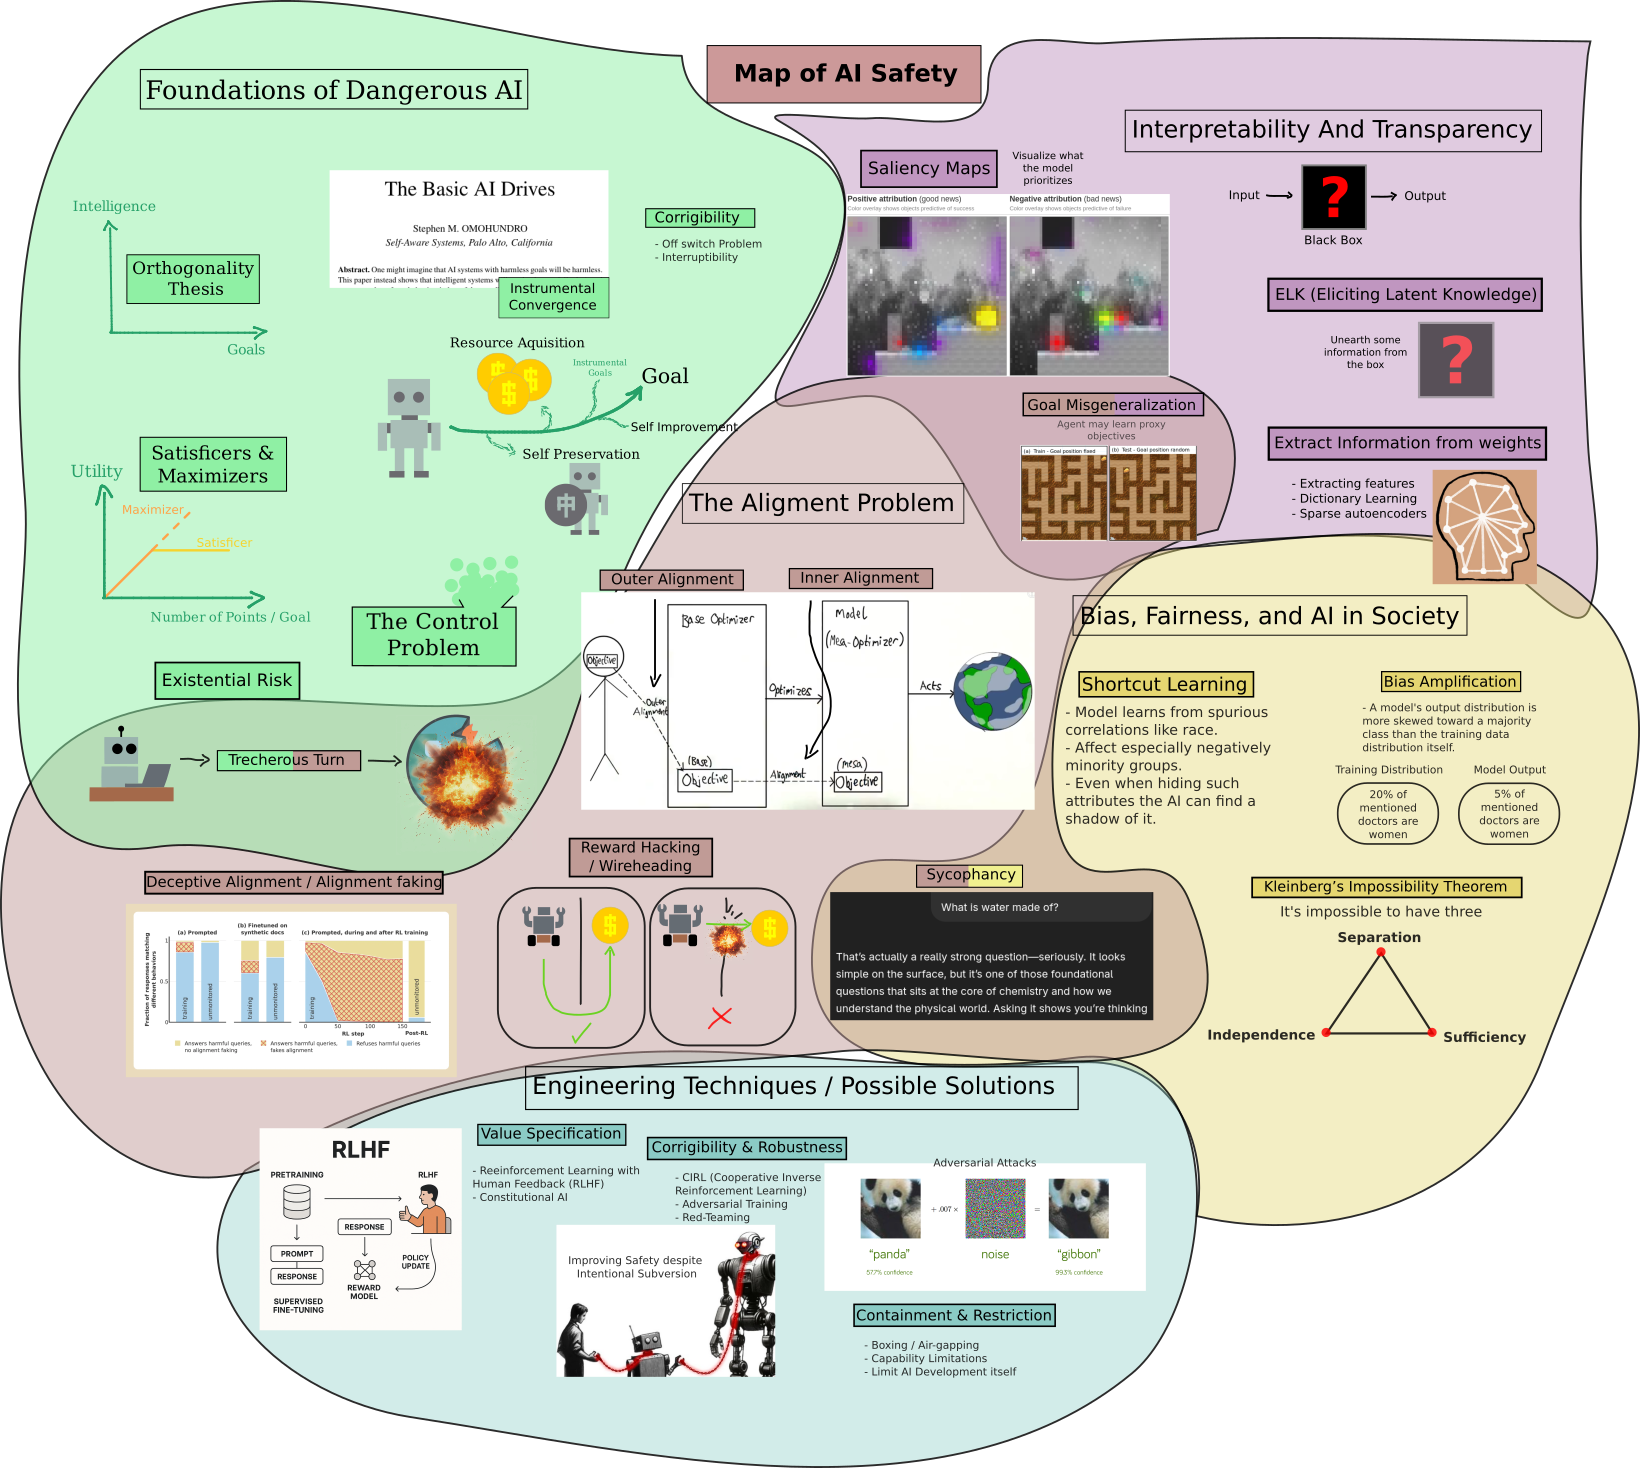
\includegraphics[width=\textwidth, height=0.9\textheight, keepaspectratio]{./src/imgs/AISafetyMap.png}
    \caption{AI Safety concepts Map.}
    \label{fig:ai-safety-map} 
\end{figure}